%%%%%%%%%%%%%%%%%%%%%%%%%%%%%%%%%%%%%%%%%
% Jacobs Landscape Poster
% LaTeX Template
% Version 1.1 (14/06/14)
%
% Created by:
% Computational Physics and Biophysics Group, Jacobs University
% https://teamwork.jacobs-university.de:8443/confluence/display/CoPandBiG/LaTeX+Poster
%
% Further modified by:
% Nathaniel Johnston (nathaniel@njohnston.ca)
%
% This template has been downloaded from:
% http://www.LaTeXTemplates.com
%
% License:
% CC BY-NC-SA 3.0 (http://creativecommons.org/licenses/by-nc-sa/3.0/)
%
%%%%%%%%%%%%%%%%%%%%%%%%%%%%%%%%%%%%%%%%%

%----------------------------------------------------------------------------------------
%	PACKAGES AND OTHER DOCUMENT CONFIGURATIONS
%----------------------------------------------------------------------------------------

\documentclass[final]{beamer}

\usepackage[scale=1.15]{beamerposter} % Use the beamerposter package for laying out the poster


\usetheme{confposter} % Use the confposter theme supplied with this template

\setbeamercolor{block title}{fg=jblue,bg=white} % Colors of the block titles
\setbeamercolor{block body}{fg=black,bg=white} % Colors of the body of blocks
\setbeamercolor{block alerted title}{fg=white,bg=dblue!70} % Colors of the highlighted block titles
\setbeamercolor{block alerted body}{fg=black,bg=dblue!10} % Colors of the body of highlighted blocks
% Many more colors are available for use in beamerthemeconfposter.sty

%-----------------------------------------------------------
% Define the column widths and overall poster size
% To set effective sepwid, onecolwid and twocolwid values, first choose how many columns you want and how much separation you want between columns
% In this template, the separation width chosen is 0.024 of the paper width and a 4-column layout
% onecolwid should therefore be (1-(# of columns+1)*sepwid)/# of columns e.g. (1-(4+1)*0.024)/4 = 0.22
% Set twocolwid to be (2*onecolwid)+sepwid = 0.464
% Set threecolwid to be (3*onecolwid)+2*sepwid = 0.708

\newlength{\sepwid}
\newlength{\onecolwid}
\newlength{\twocolwid}
\newlength{\threecolwid}
\setlength{\paperwidth}{46.8in} % A0 width: 46.8in
\setlength{\textwidth}{44.8in}
\setlength{\paperheight}{33.1in} % A0 height: 33.1in
\setlength{\textwidth}{31.1in}
\setlength{\sepwid}{0.024\paperwidth} % Separation width (white space) between columns
\setlength{\onecolwid}{0.22\paperwidth} % Width of one column
\setlength{\twocolwid}{0.464\paperwidth} % Width of two columns
\setlength{\threecolwid}{0.708\paperwidth} % Width of three columns
\setlength{\topmargin}{-0.5in} % Reduce the top margin size

%-----------------------------------------------------------


\usepackage{booktabs} % Top and bottom rules for tables

\makeatletter
\let\@@magyar@captionfix\relax
\makeatother

\usepackage{graphicx}
\usepackage{subfig}

% Matrix decomposition diagram
\usepackage{stackengine}
\stackMath
\newlength\matfield
\newlength\tmplength
\def\matscale{1.}
\newcommand\dimbox[3]{%
  \setlength\matfield{\matscale\baselineskip}%
  \setbox0=\hbox{\vphantom{X}\smash{#3}}%
  \setlength{\tmplength}{#1\matfield-\ht0-\dp0}%
  \fboxrule=1pt\fboxsep=-\fboxrule\relax%
  \fbox{\makebox[#2\matfield]{\addstackgap[.5\tmplength]{\box0}}}%
}
\newcommand\raiserows[2]{%
   \setlength\matfield{\matscale\baselineskip}%
   \raisebox{#1\matfield}{#2}%
}
\newcommand\matbox[5]{
  \stackunder{\dimbox{#1}{#2}{$#5$}}{\scriptstyle(#3\times #4)}%
}
\parskip 1em

\usepackage{siunitx} % For scientific notation of p-values using \num

\usepackage{tabularx}
% Tables with merged vertical cells
\usepackage{multirow}

\setbeamerfont{caption}{size=\footnotesize}

% set colors for alerted blocks (blocks with frame)
\setbeamercolor{block alerted title}{fg=white,bg=nred}
\setbeamercolor{block alerted body}{fg=black,bg=nred!10}

%----------------------------------------------------------------------------------------
%	TITLE SECTION
%----------------------------------------------------------------------------------------

\newcommand{\samelineand}{\qquad}

\title{Comparison of sparse biclustering algorithms for gene expression datasets} % Poster title
\author[shortname]{Katherine Nicholls \inst{1} \inst{2} and Chris Wallace \inst{1} \inst{2}}

\institute[shortinst]{\inst{1} Cambridge Institute for Therapeutic Immunology and Infectious Disease, University of Cambridge, Cambridge, CB2 0AW, UK \inst{2} MRC Biostatistics Unit, Cambridge Biomedical Campus, Forvie Site, Robinson Way, Cambridge, CB2 0SR, UK}

%----------------------------------------------------------------------------------------

\begin{document}

\addtobeamertemplate{block end}{}{\vspace*{2ex}} % White space under blocks
\addtobeamertemplate{block alerted end}{}{\vspace*{2ex}} % White space under highlighted (alert) blocks

%\setlength{\belowcaptionskip}{2ex} % White space under figures
\setlength\belowdisplayshortskip{2ex} % White space under equations


\begin{frame}[t] % The whole poster is enclosed in one beamer frame

\begin{columns}[t] % The whole poster consists of three major columns, the second of which is split into two columns twice - the [t] option aligns each column's content to the top

\begin{column}{\sepwid}\end{column} % Empty spacer column

\begin{column}{\onecolwid} % The first column

%----------------------------------------------------------------------------------------
%	INTRODUCTION
%----------------------------------------------------------------------------------------

\begin{block}{Why biclustering?}

\textbf{Groups of genes that covary} in a \textbf{subset of the samples}.

\begin{itemize}
    \item Detects patterns not visible with gene clustering
    \item Provides link between samples and gene groups
    \item Adjusts for confounders
\end{itemize}

\begin{figure}
\begin{minipage}{1\linewidth}
    \centering
\subfloat[Original matrix \label{fig:raw}]{
    
\includegraphics[width=0.2\textwidth]{plots/biclustering_diagrams/raw.png}}
\subfloat[Clustering genes\label{fig:rows}]{
    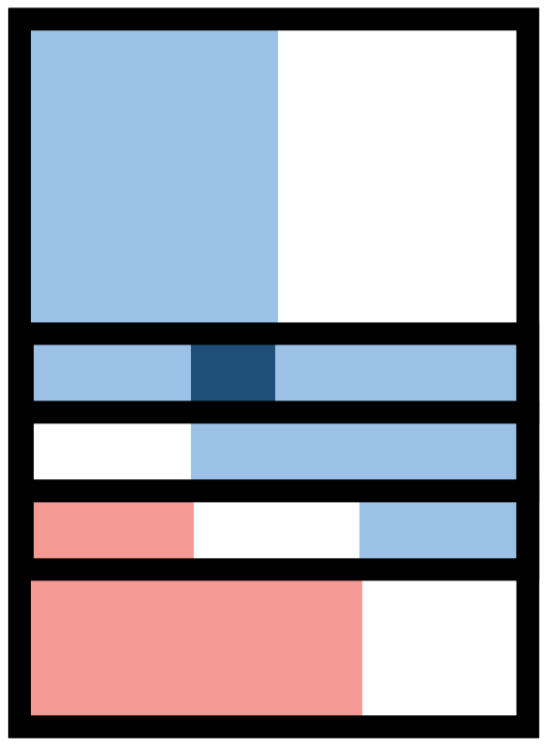
\includegraphics[width=0.2\textwidth]{plots/biclustering_diagrams/rows.png}}
\subfloat[Clustering samples\label{fig:cols}]{
    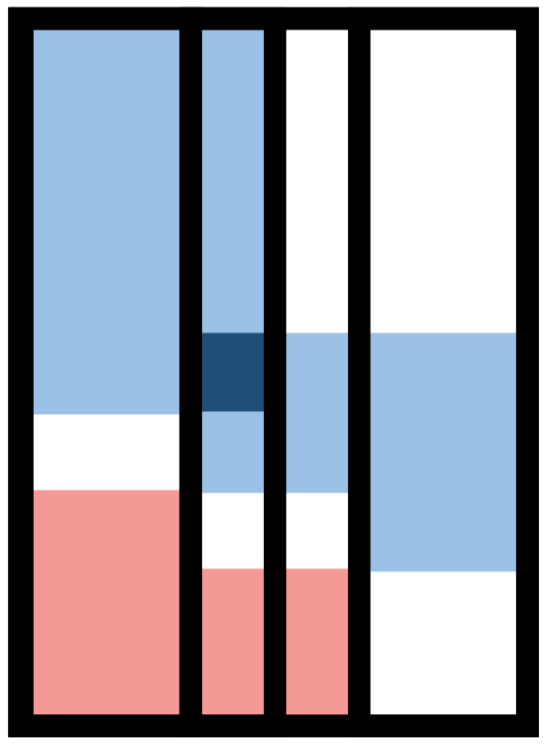
\includegraphics[width=0.2\textwidth]{plots/biclustering_diagrams/cols.png}}
\end{minipage}
\\
\begin{minipage}{1\linewidth}
    \centering
\subfloat[Biclustering\label{fig:biclusters}]{
    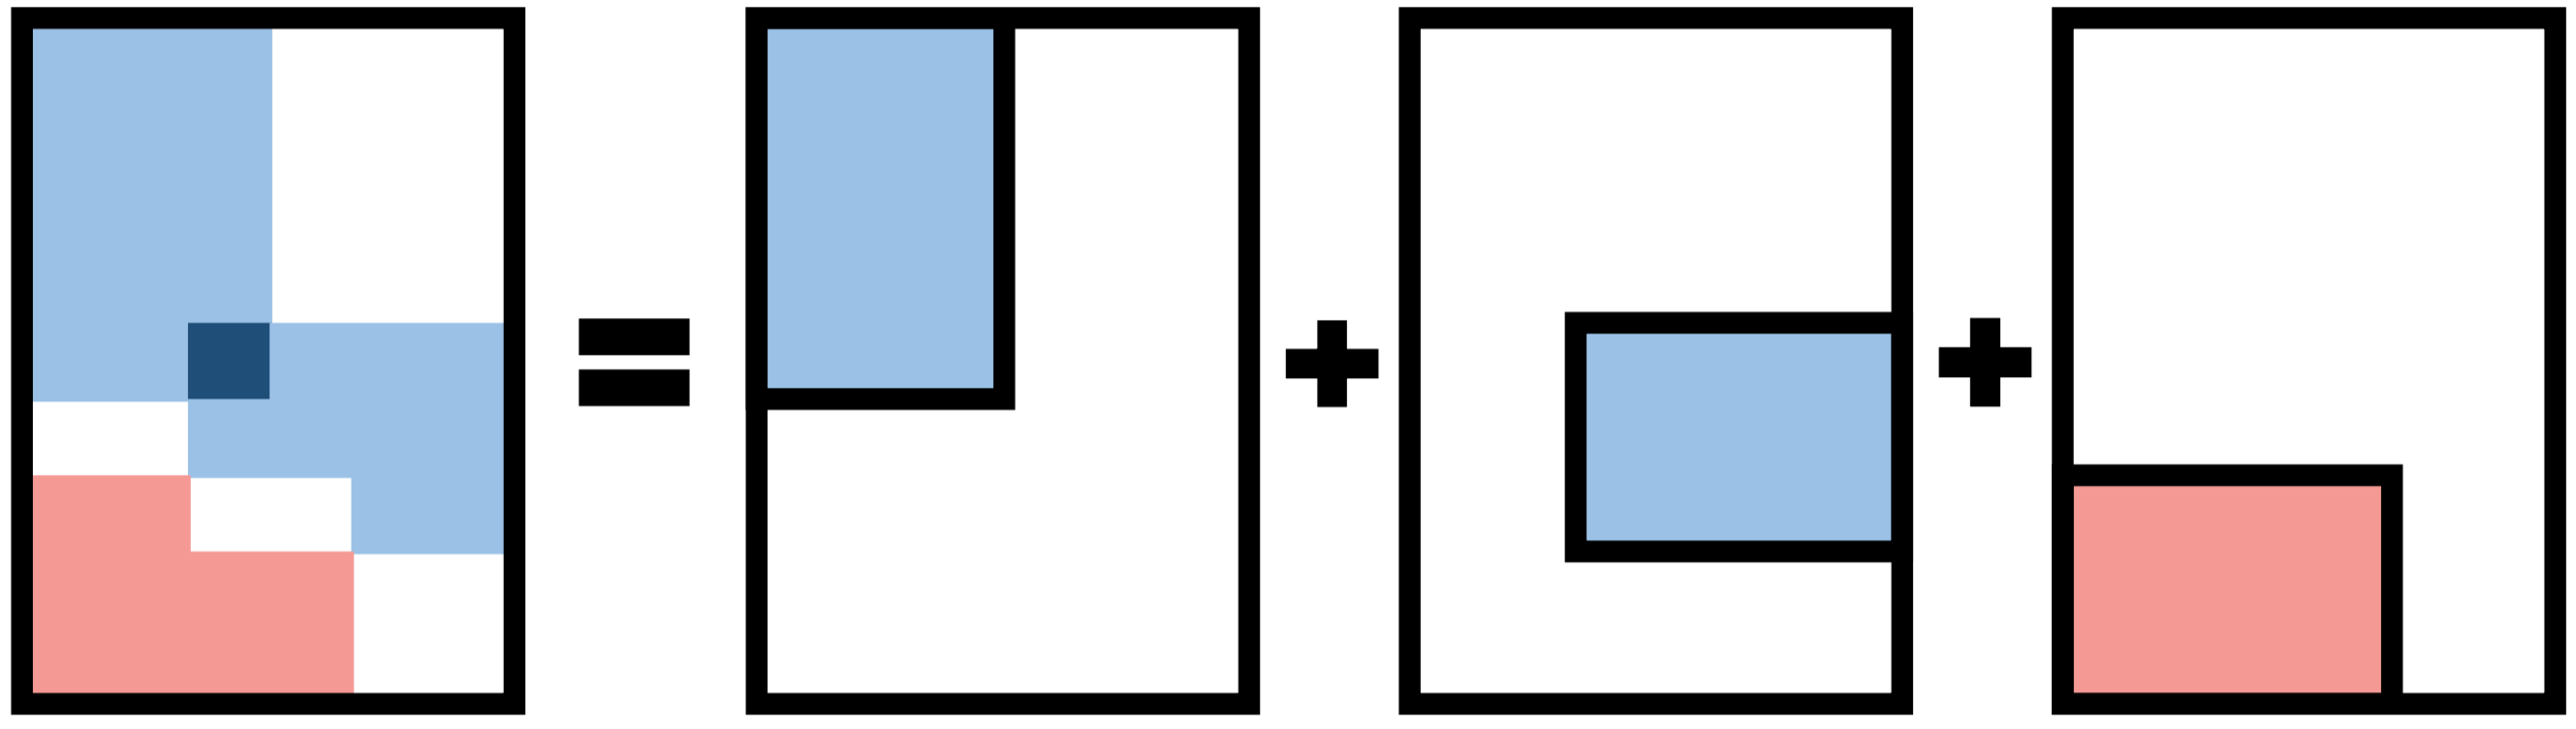
\includegraphics[width=0.85\textwidth]{plots/biclustering_diagrams/biclusters.png}}
\end{minipage}
\caption{Illustration of different kinds of clustering. The same matrix is used in each case, with rows as genes and columns as samples. Only biclustering captures the true structure of the dataset.}
\label{fig:caption}
    \end{figure}

\end{block}

%------------------------------------------------



%----------------------------------------------------------------------------------------
%	Study aims
%----------------------------------------------------------------------------------------


\begin{block}{Novel study features}

\begin{itemize}
    \item \textbf{Algorithm classes} not previously included in comparison studies
    \item \textbf{Range of complexity} of simulated datasets
    \item \textbf{Direct evaluation} of biclustering on \textbf{real datasets}
\end{itemize}

\end{block}

%----------------------------------------------------------------------------------------



%----------------------------------------------------------------------------------------
%	ALGORITHMS
%----------------------------------------------------------------------------------------

\begin{block}{Algorithm classes}

\begin{table}[t!]
    \caption{Overview of the four classes of biclustering algorithm included.}

    \begin{tabular}{ l | l }
\textbf{Class} & \textbf{Advantages} \\ \hline
\textbf{\textit{Popular}} & \multirow{2}{0.6 \textwidth}{Benchmark - in previous comparison studies} \\
     FABIA, Plaid & \\ \hline
    \textbf{\textit{NMF}} & \multirow{2}{0.6 \textwidth}{Fast, interpretable} \\
    nsNMF, SNMF & \\ \hline
    \textbf{\textit{Tensor}} & \multirow{2}{0.6 \textwidth}{Share information across cell types} \\
    MultiCluster, SDA & \\ \hline
    \textbf{\textit{Adaptive}} & \multirow{2}{0.6 \textwidth}{Mixture of sparse and dense factors, learn K automatically} \\
    BicMix, SSLB & \\ \hline
\end{tabular}
\end{table}

\end{block}

\end{column} % End of the first column

\begin{column}{\sepwid}\end{column} % Empty spacer column

\begin{column}{\onecolwid} % The second column

%----------------------------------------------------------------------------------------
%	BICMIX
%----------------------------------------------------------------------------------------



\begin{block}{Methods}

\begin{itemize}
\setlength{\itemindent}{2em}
\item{Quantified RNA-seq reads using kallisto \cite{Bray_2016}}
\item{Sparse genes discarded}
\item{Gaussian rank transformation}
\end{itemize}

\begin{figure}[h]
\centering
\includegraphics[width=\textwidth]{TSNE_allnormalisation_10nz_p30.png}
\caption{t-SNE applied to the dataset after dropping sparse genes. In each case, I applied Gaussian rank normalisation was applied and then ran PCA to find dimensions to explain $95\%$ of the variance and then ran t-SNE on this reduced set of dimensions.}
\label{fig:TSNE_allrn_p30}
\end{figure}

We use BicMix \cite{Gao_2016}, a Bayesian sparse factor analysis tool.

\begin{itemize}
\setlength{\itemindent}{2em}
\item{Sparsity-inducing prior on both $\Lambda$ and $F$}
\item{Prior is three parameter beta distribution}
\item{Each factor corresponds to a bicluster}
\item{Error is independent with gene-specific variance}
\end{itemize}

\begin{figure}[h]
\begin{center}
$\renewcommand\matscale{1.2}
\matbox{7}{4}{p}{n}{\mathrm{M}} =
\matbox{7}{2}{p}{K}{\Lambda} \raiserows{2.5}{\matbox{2}{4}{K}{n}{F}} +
\matbox{7}{4}{p}{n}{\varepsilon}$
\end{center}
\caption{Decomposition of a gene expression matrix of $p$ genes and $n$ samples using sparse factor analysis with $K$ factors.}
\end{figure}

\begin{alertblock}{}
Biclustering is a useful technique for analysing gene expression data across multiple cell types, as we expect genes to cluster differently in different cell types.
\end{alertblock}

Using samples from multiple disease types allows the model to learn how genes are co-regulated in different perturbed states.

\end{block}



%----------------------------------------------------------------------------------------

\end{column} % End of column 2

\begin{column}{\sepwid}\end{column} % Empty spacer column

\begin{column}{\onecolwid} % The third column

%----------------------------------------------------------------------------------------
%	RESULTS
%----------------------------------------------------------------------------------------

\begin{block}{Results}

Factor values cluster by cell type or disease.

\begin{figure}[h]
\centering
\includegraphics[width=\textwidth]{factor_dist_30_combined.png}
\caption{Distribution of factor 30 values. (A-B) show the distribution of $\left\lbrace F_{30,i} : i \in \left\lbrace 1 , \dots, n \right\rbrace \right\rbrace
$ grouped by cell type (A) and by condition (B).}
\label{fig:dist_30}
\end{figure}

I used Lasso regularised regression to identify important features related to each factor. I focused on the 8 factors that were linked to systemic lupus erythematosus (SLE) below the threshold \num{1e-08}.

\begin{figure}[h]
\centering
\includegraphics[scale=0.6]{regression_factors.png}
\caption{Factors linked to SLE with $p<$ \num{1e-8}. The size and colour of the dot corresponds to the p-value according to ordinary least squares performed on the features selected by Lasso regularised regression, and then adjusted using the Benjamini-Hochberg procedure to correct for multiple testing.}
\label{fig:regression_factors_SLE}
\end{figure}

I used Fisher's exact test on the genes with non-zero loading to determine association with pathways in the KEGG database. Factor 30 has a very strong association to memory B cells (CD19mem) and to plasmablasts, derived from B cells. Interestingly, the second pathway recovered for this factor is the `B cell receptor signalling' pathway with p-value \num{4.15e-06} after correcting for multiple testing.

\vspace{20px}

\begin{table}
\begin{tabularx}{\textwidth}{ | X | l | }
\hline
KEGG pathway linked to factor 30 & Significance \\ \hline
Fc gamma R-mediated phagocytosis & \num{3.53e-08} \\
B cell receptor signaling pathway & \num{4.15e-06} \\
Regulation of actin cytoskeleton & \num{1.36e-05} \\
Chemokine signaling pathway & \num{2.49e-05} \\
\hline
\end{tabularx}
\end{table}

\end{block}

%----------------------------------------------------------------------------------------

\end{column} % End of column 3

\begin{column}{\sepwid}\end{column} % Empty spacer column

\begin{column}{\onecolwid} % The fourth column

%----------------------------------------------------------------------------------------
%	CONCLUSION
%----------------------------------------------------------------------------------------

\begin{block}{Results}

Factor 10 has a strong association with SLE and AAV-MPO, and also with neutrophils (CD16FACS, CD16FACS) and monocytes (CD14).

\begin{figure}[h]
\centering
\includegraphics[width=\textwidth]{factor_dist_10_combined.png}
\caption{Distribution of factor 10 values. (A-B) show the distribution of $\left\lbrace F_{10,i} : i \in \left\lbrace 1 , \dots, n \right\rbrace \right\rbrace
$ grouped by cell type (A) and by condition (B).}
\label{fig:dist_10}
\end{figure}

The genes in factor 10 include many from the MolSigDB gene sets associated with response to viruses through interferon signalling.

\begin{table}
\begin{center}

\begin{tabularx}{\textwidth}{ | X | l | }
\hline
Gene set & Unadjusted p-value \\ \hline

Interferon gamma response &  \num{3.79e-24} \\
Interferon alpha response & \num{1.43e-19} \\

\hline
\end{tabularx}
\end{center}
\caption{MolSigDB hallmark gene sets linked to factor 10. The p-values are from Fisher's exact test.\label{tab:pathways_factor_10_int}}
\end{table}

\end{block}


\begin{block}{Conclusion}

\begin{itemize}
    \item Post-processing thresholding essential for most algorithms
    \item Adaptive algorithms best on dataset with unknown K and without processing
    \item NMF algorithms have potential - fast, robust and nsNMF performed well
    \item Little benefit found for tensor algorithms
    \item Introduced metrics for real datasets where truth is not known
\end{itemize}

\end{block}

\begin{alertblock}{Preprint}
For more details, see the preprint on bioRxiv: \\
\small \url{https://doi.org/10.1101/2020.12.15.422852}
\end{alertblock}

%----------------------------------------------------------------------------------------
%	REFERENCES
%----------------------------------------------------------------------------------------

\begin{block}{References}

\nocite{*} % Insert publications even if they are not cited in the poster
{\bibliographystyle{plain}
\bibliography{poster}}

\end{block}

%----------------------------------------------------------------------------------------
%	ACKNOWLEDGEMENTS
%----------------------------------------------------------------------------------------

\begin{center}
\begin{tabular}{ccccc}

\includegraphics[height=22mm]{./Cambridge_University_CMYK.eps} & \hspace{15mm} & 
\includegraphics[height=22mm]{mrc_logo.jpg} & \hspace{15mm} & 
\includegraphics[height=22mm]{wellcome-logo-black.jpg}
\end{tabular}
\end{center}

%----------------------------------------------------------------------------------------

\end{column} % End of the fourth column

\end{columns} % End of all the columns in the poster

\end{frame} % End of the enclosing frame

\end{document}
